%!TEX root = ../../msc17-game-book.tex

\phWorksheet{Solution - Main Puzzle 3}

Hints
\begin{itemize}
\item[*] Help the students to try drawing four of the symbols on a piece of paper in such a way that none of the lines cross. Once they've done that, see if they can draw the same picture on the inner tube, but have one of the lines wrap around the inside or back of the inner tube.
\end{itemize}

Solution

This problem is equivalent to asking one to embed a complete graph on 5 vertices ($K_5$) on the torus (or donut). A solution can be drawn on a two-dimensional rectangle where the four corners are understood to represent the same point and the sides across from each other can be wrapped around and pasted together to form the torus. There are multiple solutions to this problem, one is included here. In the picture solution below, the orange and green edges wrap around the inside or ``back'' of the torus respectively.


    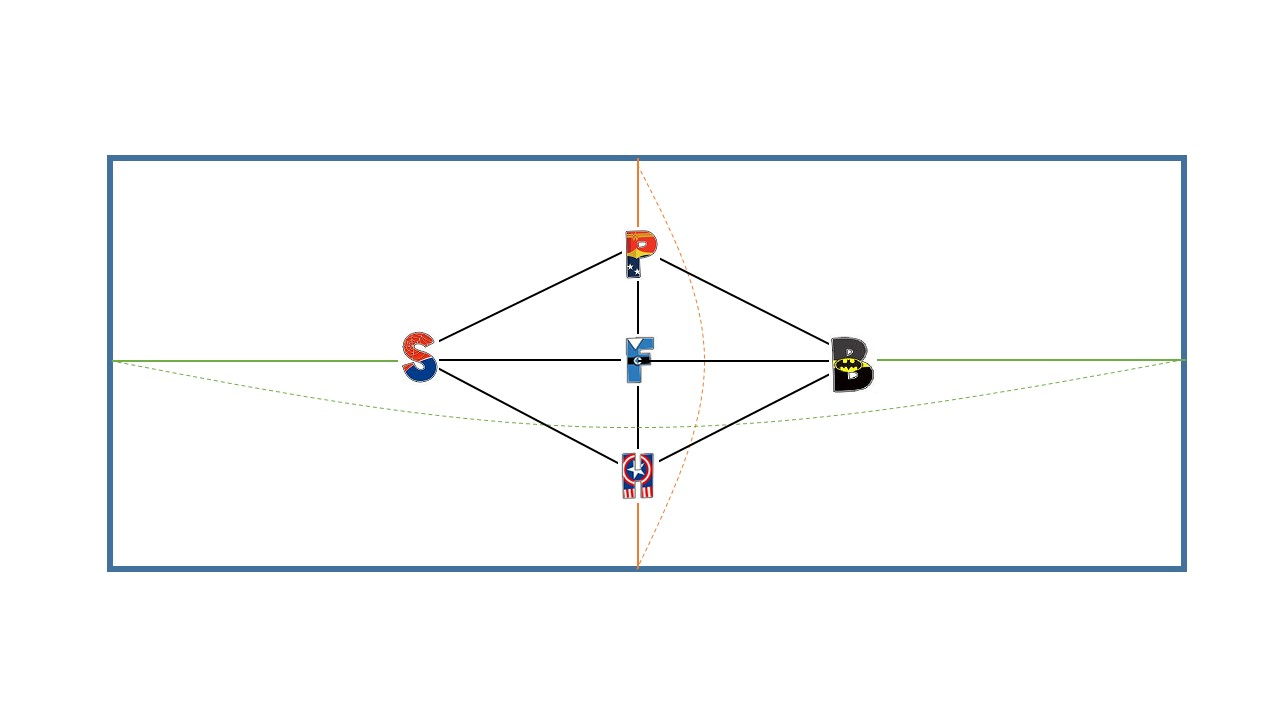
\includegraphics[width=\textwidth]{assets/kat/sol1}
